\documentclass[a4paper,12pt]{article}

\usepackage[a4paper, margin=0.9in]{geometry}
\usepackage[utf8]{inputenc}
\usepackage[T1]{fontenc}
\usepackage[polish]{babel}
\usepackage{lmodern}
\usepackage{amsmath}
\usepackage{graphicx}
\usepackage{enumitem}
\usepackage{tabularx}
\usepackage{booktabs}
\usepackage{array}
\usepackage{parskip}
\usepackage{caption}
\usepackage{float}
\usepackage{siunitx}
\usepackage{textgreek}
\usepackage[table]{xcolor}
\usepackage{hyperref}
\usepackage{titlesec}

\sisetup{
	locale = DE,
	detect-all,
	per-mode = symbol,
	separate-uncertainty = true
}

\hypersetup{
	colorlinks=true,
	linkcolor=blue,
	urlcolor=blue,
}



\usepackage{listings}
\usepackage{xcolor}

\lstdefinestyle{maxima}{
	language=,
	basicstyle=\ttfamily\small,
	keywordstyle=\color{blue},
	commentstyle=\color{gray},
	stringstyle=\color{red},
	numbers=left,
	numberstyle=\tiny,
	stepnumber=1,
	frame=single,
	breaklines=true,
	tabsize=2,
	captionpos=b
}

\lstset{style=maxima}



% Налаштування стилів розділів
\titleformat{\section}
{\LARGE\bfseries}{\thesection}{0.5em}{}

\titleformat{\subsection}
{\large\bfseries}{\thesubsection}{0.5em}{}

% Відступи для розділів
\titlespacing{\section}{0pt}{18pt}{9pt}
\titlespacing{\subsection}{0pt}{12pt}{6pt}

% Відступи для списків
\setlist[itemize,1]{label=\textbullet, leftmargin=*, itemsep=2pt, parsep=2pt}
\setlist[enumerate,1]{leftmargin=*, itemsep=4pt, parsep=2pt}

% Відступи між абзацами
\setlength{\parskip}{6pt}
\setlength{\parindent}{0pt}

\begin{document}
	
	\begin{titlepage}
		\begin{center}
			\Large
			
			% LOGO
			\begin{figure}[h]
				\centering
				
\includegraphics[height=3.2cm]{prz_pl.png}%
				\hfill
				
\includegraphics[height=3.2cm]{wmifs_pl.png}
			\end{figure}
			
			{\large\scshape Politechnika Rzeszowska}\\
			{\large im. Ignacego Łukasiewicza}\\[0.3cm]
			{\large\scshape\MakeUppercase{Wydział Matematyki i Fizyki Stosowanej}}
		\end{center}
		
		\vspace{2cm}
		
		% ===== TEMAT =====
		\begin{center}
			\rule{0.85\textwidth}{0.4pt}\\[0.6cm]
			{\Huge\bfseries Modelowanie nagrzewania silnika elektrycznego}\\[0.4cm]
			{\large z wykorzystaniem równań różniczkowych}\\[0.6cm]
			\rule{0.85\textwidth}{0.4pt}
		\end{center}
		
		% ===== PRZEDMIOT =====
		\begin{center}
			{\small Przedmiot: Równania różniczkowe}
		\end{center}
		
		\vspace{4cm}
		
		% ===== WYKONAWCY / OPIEKUN =====
		\begin{minipage}{0.45\textwidth}
			\begin{flushleft}
				\large
				\textit{Wykonawcy:}\\
				Vitalii Omeliukh [181517]\\
				Dmytro Pavlyk [181518]\\
				Grupa: 4
			\end{flushleft}
		\end{minipage}
		\hfill
		\begin{minipage}{0.45\textwidth}
			\begin{flushright}
				\large
				\textit{Opiekun projektu:}\\
				dr inż. Tomasz Stachyra
			\end{flushright}
		\end{minipage}
		
		\vfill
		\begin{center}
			{\large Rzeszów, \today}
		\end{center}
	\end{titlepage}
	
	\section{Wstęp teoretyczny}
	
	Celem projektu jest opisanie procesu nagrzewania silnika elektrycznego w czasie
	z wykorzystaniem równania różniczkowego zwyczajnego I rzędu.
	Podczas pracy silnik generuje straty mocy, które zamieniają się w ciepło,
	a jednocześnie oddaje ciepło do otoczenia. W wyniku konkurencji tych dwóch
	zjawisk temperatura silnika rośnie, a następnie dąży do wartości ustalonej.
	
	\subsection{Wyprowadzenie modelu matematycznego}
	
	Zgodnie z zasadą bilansu energii cieplnej, zmiana energii wewnętrznej obiektu
	jest równa różnicy między mocą doprowadzaną (stratami) a mocą odprowadzaną
	do otoczenia. Przyjmujemy uproszczony model skupiony, w którym cały silnik
	ma jednorodną temperaturę $T(t)$.
	
	Wprowadzamy następujące wielkości:
	\begin{itemize}
		\item $T(t)$ -- temperatura silnika,
		\item $T_a$ -- temperatura otoczenia,
		\item $P$ -- moc strat cieplnych silnika [W],
		\item $R_{th}$ -- rezystancja termiczna [K/W],
		\item $C_{th}$ -- pojemność cieplna [J/K].
	\end{itemize}
	
	Moc odprowadzana do otoczenia w liniowym modelu wymiany ciepła jest proporcjonalna
	do różnicy temperatur:
	\[
	P_{\text{out}} = \frac{T(t)-T_a}{R_{th}}.
	\]
	
	Zmiana energii wewnętrznej jest opisana przez pojemność cieplną:
	\[
	P_{\text{in}} - P_{\text{out}} = C_{th}\frac{dT(t)}{dt}.
	\]
	
	Ponieważ moc doprowadzana jest równa stratom $P$, otrzymujemy równanie bilansu:
	\[
	C_{th}\frac{dT(t)}{dt} = P - \frac{T(t)-T_a}{R_{th}}.
	\]
	
	\newpage
	
	\subsection{Rozwiązanie analityczne równania}
	
	Wprowadzamy przyrost temperatury względem otoczenia:
	\[
	\theta(t) = T(t) - T_a.
	\]
	
	Po podstawieniu $T(t)=\theta(t)+T_a$ otrzymujemy:
	\[
	C_{th}\frac{d\theta(t)}{dt} = P - \frac{\theta(t)}{R_{th}}.
	\]
	
	Dzieląc stronami przez $C_{th}$ i wprowadzając stałą czasową
	\[
	\tau = R_{th}C_{th},
	\]
	dostajemy standardową postać:
	\[
	\frac{d\theta}{dt} + \frac{1}{\tau}\theta = \frac{P}{C_{th}}.
	\]
	
	Rozwiązanie ogólne przy warunku początkowym $T(0)=T_0$ (czyli $\theta(0)=T_0-T_a$)
	ma postać:
	\[
	\theta(t)=PR_{th} + \bigl((T_0-T_a)-PR_{th}\bigr)e^{-t/\tau}.
	\]
	
	Zatem temperatura silnika w funkcji czasu:
	\[
	T(t)=T_a+PR_{th} + (T_0-T_a-PR_{th})e^{-t/\tau}.
	\]
	
	Temperatura ustalona (dla $t\to\infty$) wynosi:
	\[
	T_{\infty}=\lim_{t\to\infty}T(t)=T_a+PR_{th}.
	\]
	
	
	\newpage
	\section{Analiza symulacyjna w programie Maxima}
	
	Do rozwiązania problemu wykorzystano środowisko \texttt{wxMaxima}. 
	Projekt polega na modelowaniu nagrzewania silnika elektrycznego z wykorzystaniem
	Rownania różniczkowego I rzędu, opisującego bilans energii cieplnej.
	Celem symulacji było zbadanie wpływu mocy strat cieplnych $P$ (związanej z obciążeniem silnika)
	na przebieg temperatury w czasie oraz na wartość temperatury ustalonej.
	
	\subsection{Metodologia obliczeń}
	
	W programie zdefiniowano podstawowe parametry modelu termicznego:
	pojemność cieplną $C_{th}$, rezystancję termiczną $R_{th}$, temperaturę otoczenia $T_a$
	oraz moc strat cieplnych $P$ (badany parametr).
	Następnie zapisano i rozwiązano równanie różniczkowe opisujące zmianę temperatury silnika:
	
	\[
	C_{th}\frac{dT(t)}{dt} = P - \frac{T(t)-T_a}{R_{th}}.
	\]
	
	Równanie zostało rozwiązane symbolicznie przy pomocy funkcji \texttt{ode2},
	a następnie wyznaczono rozwiązanie szczególne dla zadanych warunków początkowych
	za pomocą polecenia \texttt{ic1}.  
	Do wizualizacji wyników wykorzystano funkcję \texttt{wxdraw2d}, która umożliwia
	rysowanie wykresów zależności temperatury od czasu.
	
	
	
	%	-->	/* Definicja głównego równania bilansu energii cieplnej  */;
	%	-->	equation : C*'diff(T,t) = P - (T - Ta)/R;
	%	(equation)	C·('diff(T,t,1))=P-(T-Ta)/R
	%	-->	/* Rozwiązanie ogólne równania różniczkowego */;
	%	-->	general_solution : ode2(equation, T, t);
	%	(general_solution)	T=%e^(-(t/(C·R)))·(%e^(t/(C·R))·(Ta+P·R)+%c)
	%	-->	/* Rozwiązanie szczególne z warunku początkowego */;
	%	-->	particular_solution : ic1(general_solution, t=0, T=T0);
	%	(particular_solution)	T=%e^(-(t/(C·R)))·((%e^(t/(C·R))-1)·Ta+T0+
	%	(%e^(t/(C·R))-1)·P·R)
	%	-->	/* Uproszczenie otrzymanego rozwiązania */;
	%	-->	simplified_solution : ratsimp(particular_solution);
	%	(simplified_solution)	T=%e^(-(t/(C·R)))·((%e^(t/(C·R))-1)·Ta+T0+
	%	(%e^(t/(C·R))-1)·P·R)
	%	-->	fpprintprec:5;
	%	(fpprintprec)	5
	%	-->	define(T_general(t, R, C, Ta, T0, P), rhs(simplified_solution));
	%	(%o6)	T_general(t,R,C,Ta,T0,P):=%e^(-(t/(C·R)))·((%e^(t/(C·R))-1)·Ta+T0+
	%	(%e^(t/(C·R))-1)·P·R)
	%	-->	T_specific(Ta_in, T0_in, R_in, C_in, P_in):=
	%	T(n)=float(expand(subst([Ta = Ta_in, T0 = T0_in, R=R_in, C=C_in, P=P_in], 
	%	%e^(-(t/(C*R)))*((%e^(t/(C*R))-1)*Ta+T0+(%e^(t/(C*R))-1)*P*R))));
	%	(%o7)	T_specific(Ta_in,T0_in,R_in,C_in,P_in):=T(n)=float(expand(subst([Ta=
	%	Ta_in,T0=T0_in,R=
	%	R_in,C=C_in,P=P_in],
	%	%e^(-(t/(C·R)))·((%e^(t/(C·R))-1)·Ta+T0+
	%	(%e^(t/(C·R))-1)·P·R))))
	
	
	
	\subsection{Rozwiązanie równania bilansu cieplnego w programie Maxima}
	
	W pierwszym kroku w środowisku \texttt{wxMaxima} zapisano równanie bilansu energii
	cieplnej silnika w postaci równania różniczkowego pierwszego rzędu.
	Równanie to opisuje zmianę temperatury silnika w czasie w wyniku strat mocy
	oraz wymiany ciepła z otoczeniem.
	
	Następnie równanie zostało rozwiązane symbolicznie przy pomocy funkcji
	\texttt{ode2}. Stała całkowania została wyznaczona na podstawie warunku
	początkowego $T(0)=T_0$ z wykorzystaniem polecenia \texttt{ic1}.
	Otrzymane rozwiązanie uproszczono i zapisano w postaci funkcji ogólnej
	$T(t)$.
	
	W celu wygodnego obliczania przebiegów temperatury dla konkretnych wartości
	parametrów modelu wprowadzono dodatkową funkcję \texttt{T\_specific},
	która automatycznie podstawia wartości parametrów fizycznych
	i przekształca rozwiązanie do postaci numerycznej, możliwej do bezpośredniego
	wykorzystania przy rysowaniu wykresów.
	
	\begin{lstlisting}[caption={Rozwiązanie analityczne równania bilansu cieplnego w Maxima}]
		/* Definicja rownania bilansu energii cieplnej */
		equation : C*'diff(T,t) = P - (T - Ta)/R;
		
		/* Rozwiazanie ogolne rownania rozniczkowego */
		general_solution : ode2(equation, T, t);
		
		/* Uwzglednienie warunku poczatkowego */
		particular_solution : ic1(general_solution, t=0, T=T0);
		
		/* Uproszczenie rozwiazania */
		simplified_solution : ratsimp(particular_solution);
		
		/* Definicja funkcji ogolnej T(t) */
		define(T_general(t,R,C,Ta,T0,P), rhs(simplified_solution));
		
		/* Funkcja pomocnicza do podstawiania parametrow */
		T_specific(Ta_in, T0_in, R_in, C_in, P_in) :=
		T(n) = float(
			expand(
				subst([Ta=Ta_in, T0=T0_in, R=R_in, C=C_in, P=P_in],
				%e^(-(t/(C*R))) *
				((%e^(t/(C*R))-1)*Ta + T0 + (%e^(t/(C*R))-1)*P*R)
				)
			)
		);
	\end{lstlisting}
	
	
	
	\vspace{-0.3cm}
	\subsection{Procedura obliczeniowa}
	
	Symulację przeprowadzono w następujących krokach:
	
	\begin{enumerate}
		\item \textbf{Definicja równania} – zapisanie równania różniczkowego z użyciem składni Maxima.
		\item \textbf{Rozwiązanie analityczne} – użycie funkcji \texttt{ode2} do uzyskania rozwiązania ogólnego.
		\item \textbf{Uwzględnienie warunku początkowego} – zastosowanie \texttt{ic1} dla $T(0) = T_0$.
		\item \textbf{Podstawienie parametrów} – obliczenie konkretnych przebiegów dla każdego scenariusza.
		\item \textbf{Wizualizacja} – generacja wykresów za pomocą \texttt{wxdraw2d}.
		\item \textbf{Analiza wyników} – porównanie temperatur ustalonych i czasów nagrzewania.
	\end{enumerate}
	
	
	
	
	%	 -->	/* Przykładowe wartości parametrów */;
	%	-->	Ta11: 20$;      /* temperatura otoczenia */
	%	T011: 20$;      /* temperatura początkowa silnika */
	%	R11 : 2$;       /* rezystancja termiczna */
	%	C11: 5$;       /* pojemność cieplna */
	%	/* Dwie różne moce strat – małe i duże obciążenie */
	%	P11: 50$;
	%	P12: 150$;
	%	-->	define(W11(t),rhs(T_specific(Ta11, T011, R11, C11, P11)));
	%	(%o14)	W11(t):=120.0-100.0/2.7183^(t/10)
	%	-->	define(W12(t),rhs(T_specific(Ta11, T011, R11, C11, P12)));
	%	(%o15)	W12(t):=320.0-300.0/2.7183^(t/10)
	%	-->	/* Wykres */;
	%	-->	wxdraw2d(
	%	xlabel = "Czas t",
	%	ylabel = "Temperatura T(t)",
	%	key = "Mała moc strat (P=50 W)",
	%	explicit(W11(t), t, 0, 50),
	%	
	%	color = red,
	%	key =  "Duża moc strat (P=150 W)",
	%	explicit(W12(t), t, 0, 50),
	%	color = blue
	%	);
	%	(%t16)	 (Graphics) 
	%	(%o16)	
	
	
	
	\subsection{Wybrane scenariusze symulacyjne}
	
	W celu analizy wpływu obciążenia silnika na jego nagrzewanie rozpatrzono trzy przypadki,
	odpowiadające różnym poziomom mocy strat cieplnych:
	
	\textbf{Scenariusz : Małe/Duże obciążenie silnika}
	\begin{itemize}
		\item Temperatura otoczenia: $T_a = 20^\circ C$,
		\item Temperatura początkowa: $T_0 = 20^\circ C$,
		\item Rezystancja termiczna: $R_{th} = 0.2 \ \mathrm{K/W}$,
		\item Pojemność cieplna: $C_{th} = 1000 \ \mathrm{J/K}$,
		\item Moc strat: $P = 50 \ \mathrm{W}$.
	\end{itemize}
	
	
	Przyjęcie trzech różnych wartości mocy strat pozwala na bezpośrednie porównanie,
	w jaki sposób zmiana obciążenia wpływa na temperaturę ustaloną silnika
	oraz na czas osiągnięcia stanu quasi-stacjonarnego.
	Stała czasowa nagrzewania $\tau = R_{th}C_{th} = 200$ s jest identyczna we wszystkich przypadkach,
	co pozwala wyizolować wpływ samego parametru $P$.
	
	\begin{figure}[h!]
		\centering
		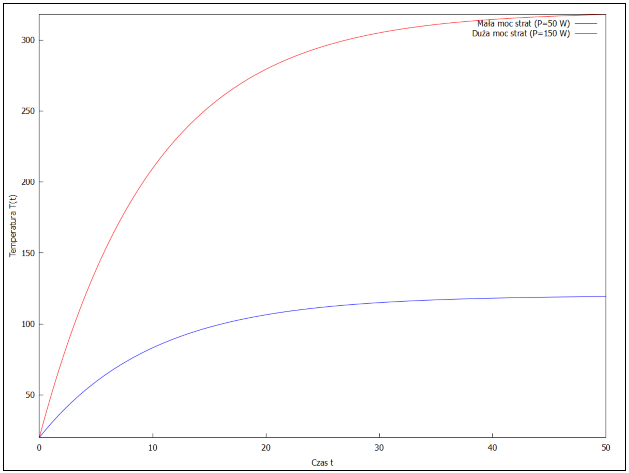
\includegraphics[width=0.75\textwidth]{WYKRES1.png}
		\caption{Przebieg temperatury silnika $T(t)$ w czasie dla różnych wartości mocy strat $P$.}
		\label{fig:temp_silnika}
	\end{figure}
	
	
	
	%	 -->	/* Przykładowe wartości parametrów */;
	%	-->	Ta11: 20$;      /* temperatura otoczenia */
	%	T011: 20$;      /* temperatura początkowa silnika */
	%	R11 : 2$;       /* rezystancja termiczna */
	%	C11: 5$;       /* pojemność cieplna */
	%	/* Dwie różne moce strat – małe i duże obciążenie */
	%	P11: 50$;
	%	P12: 150$;
	%	-->	define(W11(t),rhs(T_specific(Ta11, T011, R11, C11, P11)));
	%	(%o14)	W11(t):=120.0-100.0/2.7183^(t/10)
	%	-->	define(W12(t),rhs(T_specific(Ta11, T011, R11, C11, P12)));
	%	(%o15)	W12(t):=320.0-300.0/2.7183^(t/10)
	%	-->	/* Wykres */;
	%	-->	wxdraw2d(
	%	xlabel = "Czas t",
	%	ylabel = "Temperatura T(t)",
	%	key = "Mała moc strat (P=50 W)",
	%	explicit(W11(t), t, 0, 50),
	%	
	%	color = red,
	%	key =  "Duża moc strat (P=150 W)",
	%	explicit(W12(t), t, 0, 50),
	%	color = blue
	%	);
	%	(%t16)	 (Graphics) 
	%	(%o16)	
	
	
	\subsection{Wpływ mocy strat na przebieg temperatury w czasie}
	
	W celu analizy wpływu obciążenia silnika na proces nagrzewania
	rozpatrzono dwa przypadki odpowiadające małej i dużej mocy strat cieplnych.
	Pozostałe parametry modelu pozostały niezmienne.
	
	Dla każdej wartości mocy strat obliczono przebieg temperatury w czasie
	na podstawie rozwiązania analitycznego i przedstawiono go graficznie.
	
	\begin{lstlisting}[caption={Definicja parametrów i wykres temperatury w czasie}]
		Ta11 : 20$      /* temperatura otoczenia */
		T011: 20$       /* temperatura poczatkowa */
		R11 : 2$        /* rezystancja termiczna */
		C11 : 5$        /* pojemnosc cieplna */
		
		/* Dwie moce strat */
		P11 : 50$
		P12 : 150$
		
		define(W11(t), rhs(T_specific(Ta11,T011,R11,C11,P11)));
		define(W12(t), rhs(T_specific(Ta11,T011,R11,C11,P12)));
		
		wxdraw2d(
		xlabel = "Czas t",
		ylabel = "Temperatura T(t)",
		key = "P = 50 W",
		color = red,
		explicit(W11(t), t, 0, 50),
		key = "P = 150 W",
		color = blue,
		explicit(W12(t), t, 0, 50)
		);
	\end{lstlisting}
	
	
	
	\subsection{Temperatura ustalona silnika w funkcji mocy strat i rezystancji termicznej}
	
	Z analitycznego rozwiązania równania bilansu cieplnego wynika, że temperatura ustalona
	silnika zależy liniowo od mocy strat $P$ oraz rezystancji termicznej $R_{th}$ i jest dana wzorem:
	\[
	T_\infty = T_a + P R_{th}.
	\]
	Oznacza to, że zarówno wzrost obciążenia silnika (zwiększenie mocy strat),
	jak i pogorszenie warunków odprowadzania ciepła (wzrost rezystancji termicznej)
	prowadzą do podwyższenia temperatury pracy silnika.
	
	W celu zilustrowania tej zależności wykonano wykres temperatury ustalonej $T_\infty$
	w funkcji mocy strat $P$ dla różnych wartości rezystancji termicznej $R_{th}$.
	Analiza została przeprowadzona w sposób parametryczny z wykorzystaniem suwaka,
	co umożliwia dynamiczną zmianę wartości $R_{th}$.
	
	Przyjęto następujące wartości:
	\begin{itemize}
		\item Temperatura otoczenia: $T_a = 20^\circ C$,
		\item Zakres mocy strat: $P \in [0,\ 120]\ \mathrm{W}$,
		\item Rezystancja termiczna:
		\[
		R_{th} \in \{0.5,\; 1,\; 2,\; 4,\; 8,\; 16\}\ \mathrm{K/W}.
		\]
	\end{itemize}
	
	Dla każdej wartości rezystancji termicznej wykreślono słupkową charakterystykę
	temperatury ustalonej w funkcji mocy strat.
	Zmiana wartości $R_{th}$ realizowana jest interaktywnie za pomocą suwaka,
	co pozwala na bezpośrednie porównanie wpływu warunków chłodzenia
	na temperaturę ustaloną silnika.
	
	\begin{figure}[h!]
		\centering
		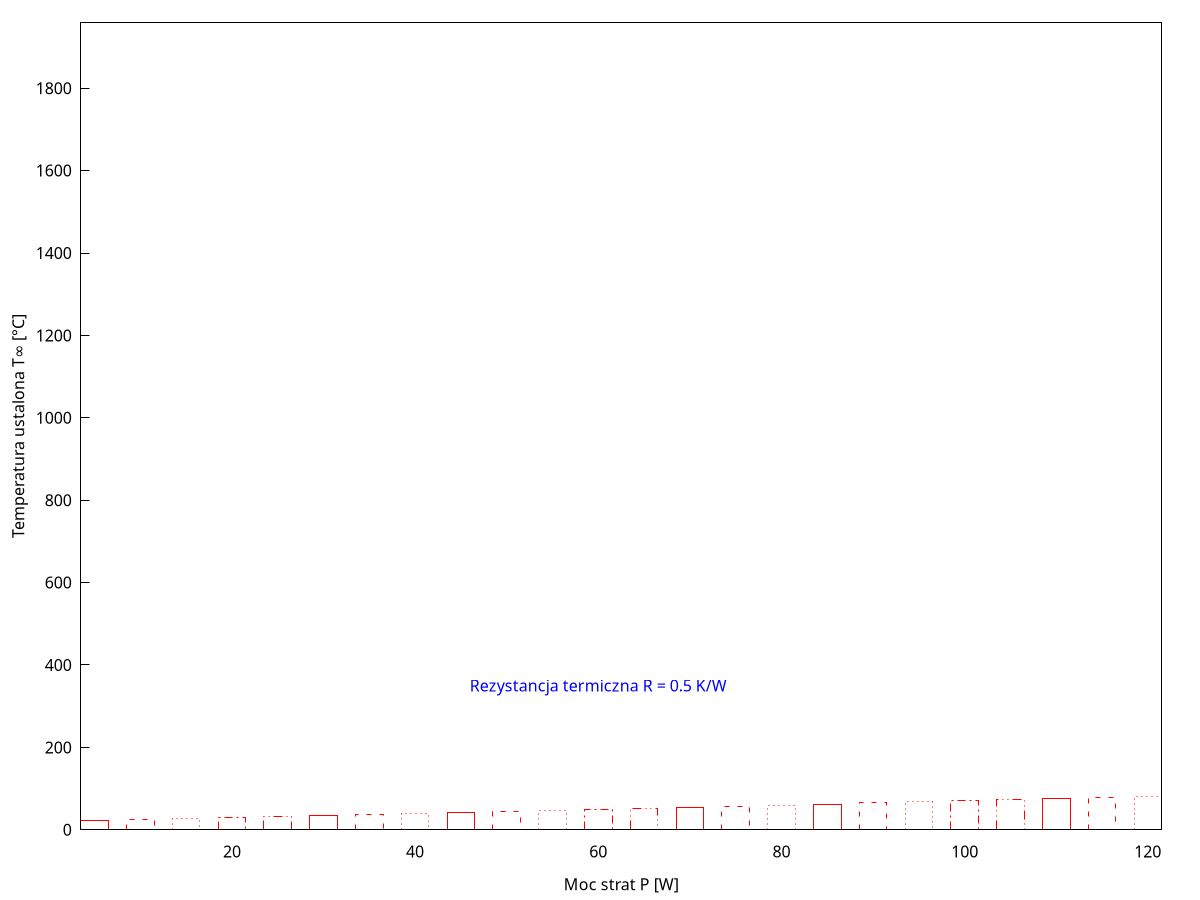
\includegraphics[width=0.45\textwidth]{WYKRES2_1.png}
		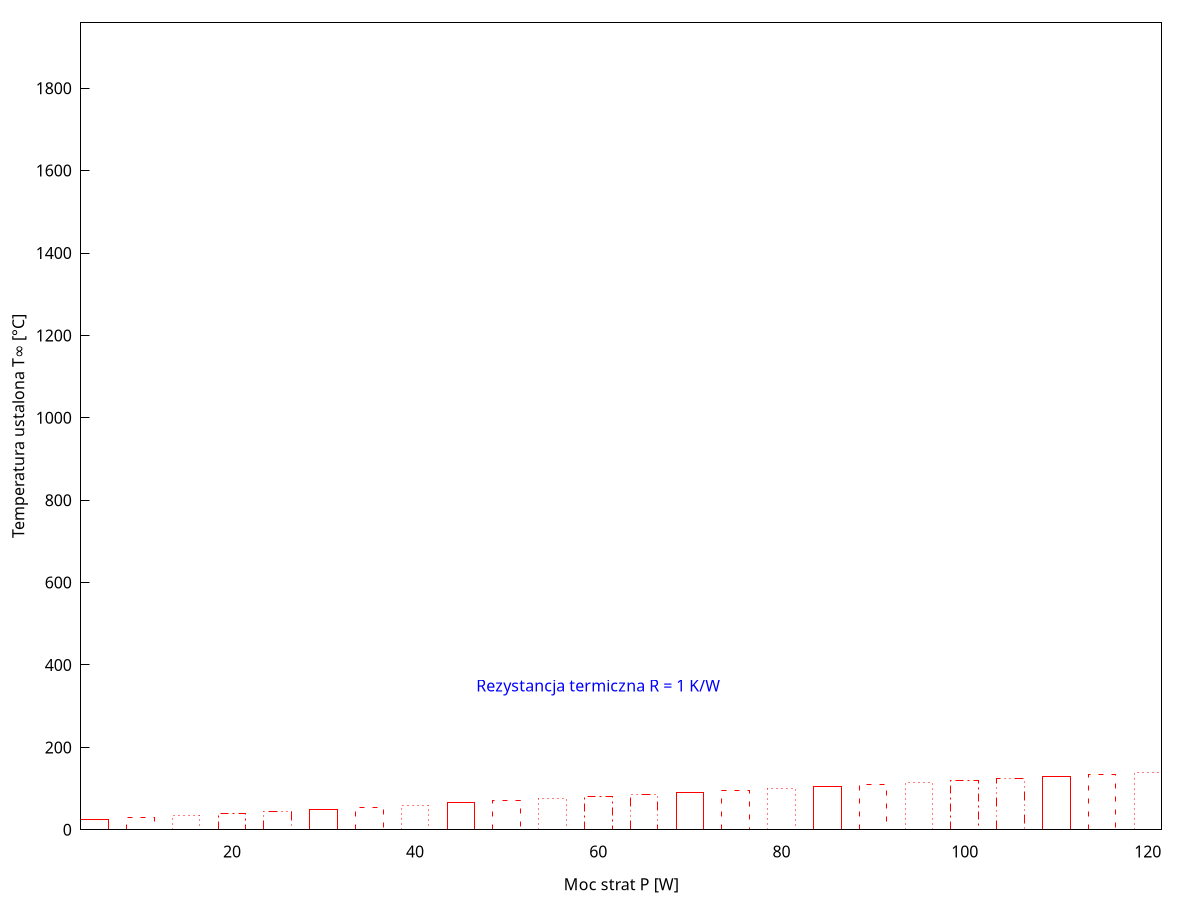
\includegraphics[width=0.45\textwidth]{WYKRES2_2.png}
		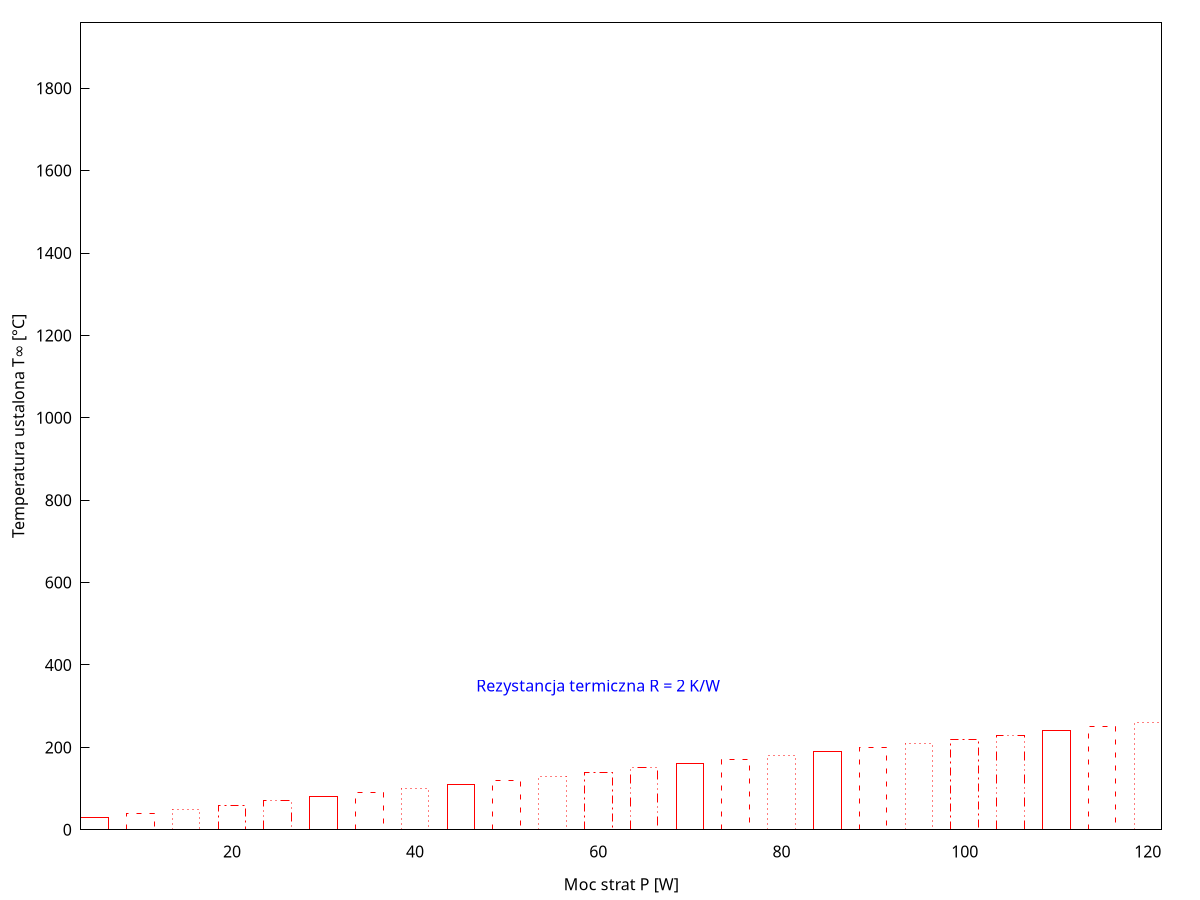
\includegraphics[width=0.45\textwidth]{WYKRES2_3.png}
		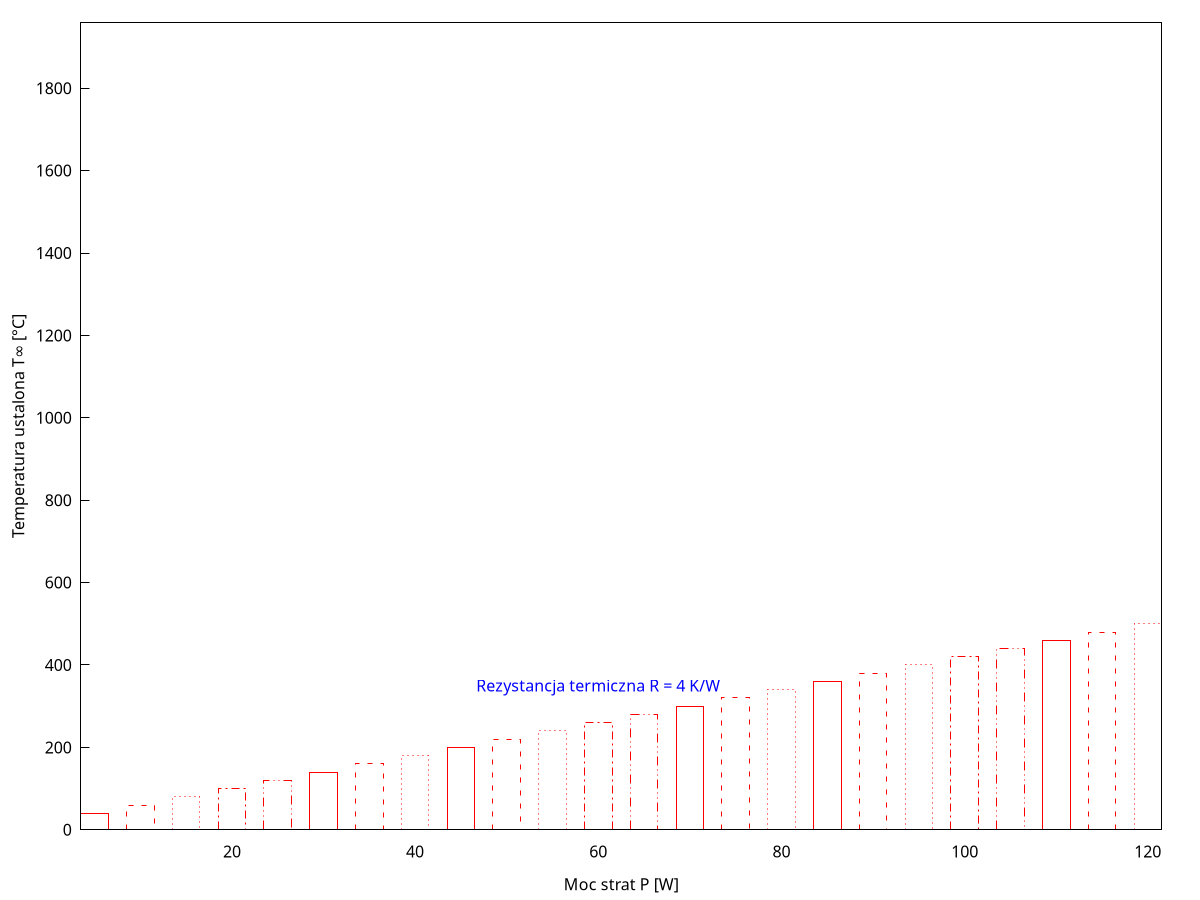
\includegraphics[width=0.45\textwidth]{WYKRES2_4.png}
		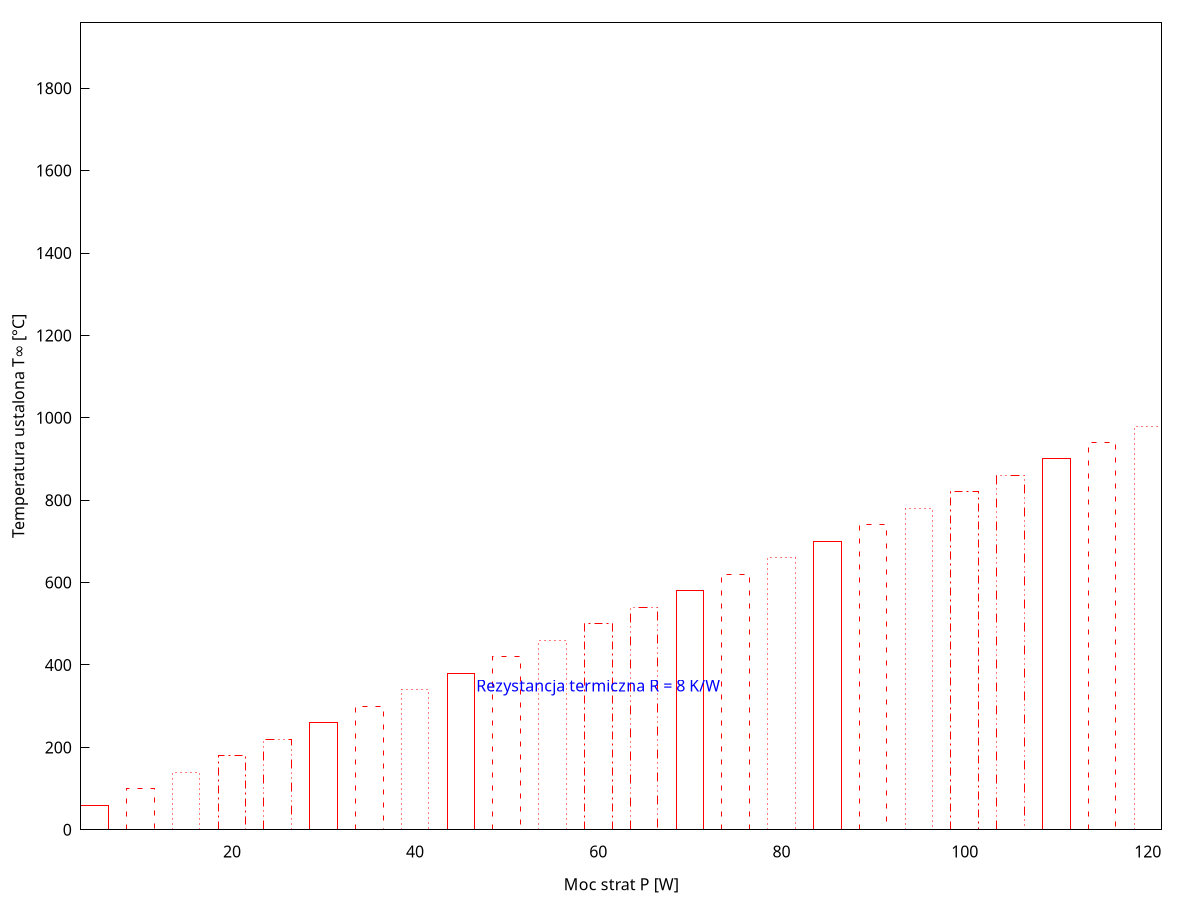
\includegraphics[width=0.45\textwidth]{WYKRES2_5.png}
		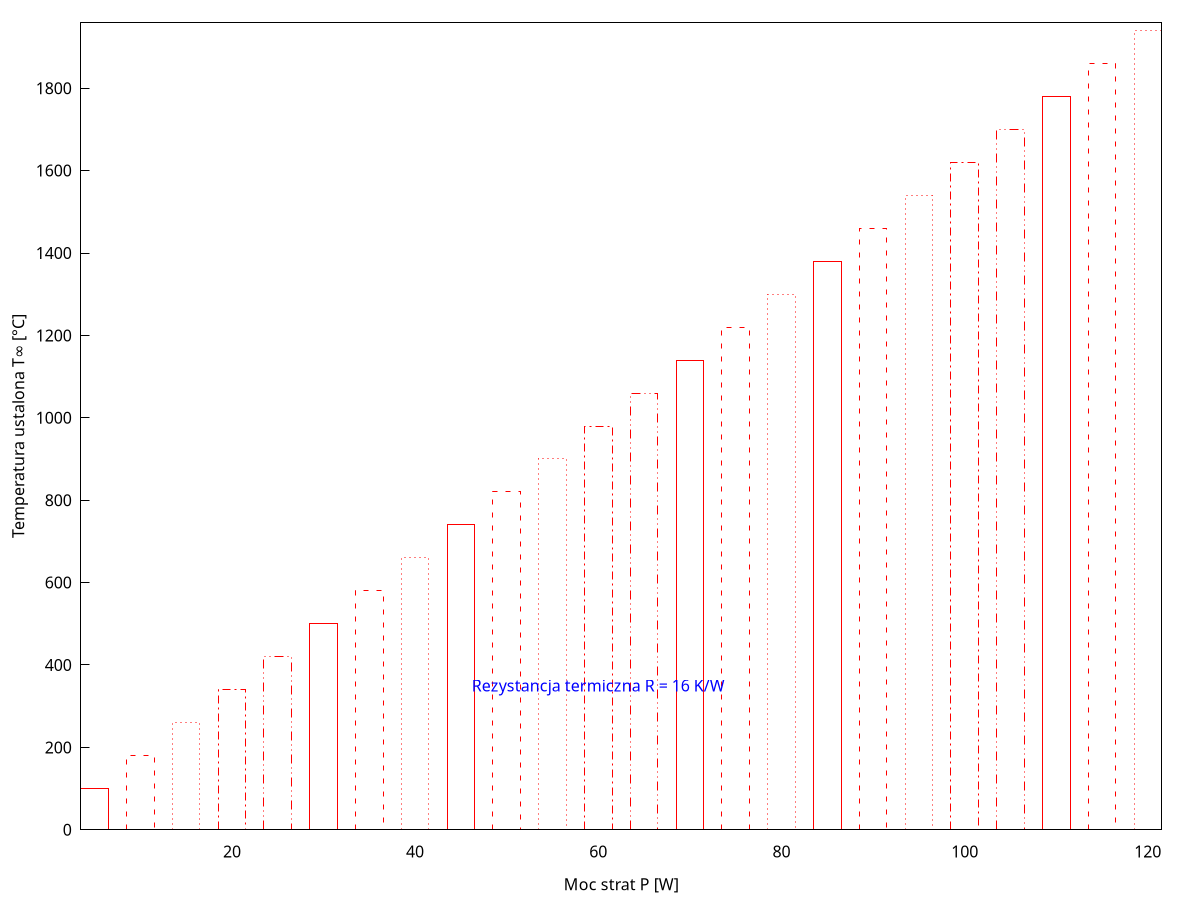
\includegraphics[width=0.45\textwidth]{WYKRES2_6.png}
		
		\caption{Zależność temperatury ustalonej $T_\infty(P)$
			dla różnych wartości rezystancji termicznej $R_{th}$.}
		\label{fig:TinfP_R}
	\end{figure}
	
	Na rysunku widoczna jest liniowa zależność temperatury ustalonej od mocy strat
	dla każdej wartości $R_{th}$.
	Jednocześnie wraz ze wzrostem rezystancji termicznej nachylenie charakterystyki
	rośnie, co oznacza większą wrażliwość temperatury silnika na zmiany obciążenia.
	Potwierdza to fizyczną interpretację parametru $R_{th}$ jako miary skuteczności
	odprowadzania ciepła do otoczenia.
	
	
	
	
	%	 -->	/* Parametry stałe */
	%	Ta31 : 20$      /* temperatura otoczenia */
	%	T031 : 20$      /* temperatura początkowa */
	%	R31  : 2$       /* rezystancja termiczna */
	%	P31  : 100$     /* stała moc strat */
	%	/* Różne pojemności cieplne */
	%	C31 : 2$
	%	C32 : 5$
	%	C33 : 10$
	%	-->	define(W31(t),rhs(T_specific(Ta31, T031, R31, C31, P31)));
	%	(%o32)	W31(t):=220.0-200.0/2.7183^(t/4)
	%	-->	define(W32(t),rhs(T_specific(Ta31, T031, R31, C32, P31)));
	%	(%o33)	W32(t):=220.0-200.0/2.7183^(t/10)
	%	-->	define(W33(t),rhs(T_specific(Ta31, T031, R31, C33, P31)));
	%	(%o34)	W33(t):=220.0-200.0/2.7183^(t/20)
	%	-->	/* Wykres z kolorami i opisami */
	%	wxdraw2d(
	%	xlabel = "Czas t",
	%	ylabel = "Temperatura T(t)",
	%	yrange = [20, 250],
	%	
	%	key = "C_th = 2 J/K",
	%	color = red,
	%	explicit(W31(t), t, 0, 50),
	%	
	%	key = "C_th = 5 J/K",
	%	color = blue,
	%	explicit(W32(t), t, 0, 50),
	%	
	%	key = "C_th = 10 J/K",
	%	color = green,
	%	explicit(W33(t), t, 0, 50)
	%	);
	%	(%t35)	 (Graphics) 
	%	(%o35)	
	
	
	
	\subsection{Parametryczna analiza temperatury ustalonej}
	
	Z zależności analitycznej wynika, że temperatura ustalona silnika
	jest funkcją liniową zarówno mocy strat $P$, jak i rezystancji termicznej $R_{th}$.
	Aby zilustrować wpływ warunków chłodzenia, przeprowadzono analizę
	parametryczną dla kilku wartości $R_{th}$.
	
	Wykorzystano mechanizm suwaka programu \texttt{wxMaxima}, który umożliwia
	dynamiczną zmianę wartości rezystancji termicznej i obserwację wpływu
	na temperaturę ustaloną.
	
	\begin{lstlisting}[caption={Temperatura ustalona w funkcji P i Rth}]
		Ta21 : 20$
		Tinf(P,R) := Ta21 + P*R$
		
		Pvals : makelist(5*i, i, 1, 24)$
		Rvals : [0.5,1,2,4,8,16]$
		dP : 3$
		
		with_slider_draw(
		R, Rvals,
		xlabel = "Moc strat P [W]",
		ylabel = "Temperatura ustalona T_inf [C]",
		color = blue,
		makelist(
		bars([Pvals[i], Tinf(Pvals[i],R), dP]),
		i,1,length(Pvals)
		),
		label([concat("R_th = ",R," K/W"), 60, 350])
		);
	\end{lstlisting}
	
	
	
	\newpage
	\subsection{Wpływ pojemności cieplnej $C_{th}$ na nagrzewanie silnika}
	
	Kolejnym analizowanym parametrem była pojemność cieplna $C_{th}$, opisująca zdolność
	silnika do magazynowania energii cieplnej. Wpływa ona na dynamikę procesu nagrzewania.
	
	Rozpatrzono trzy wartości:
	\[
	C_{th} \in \{2,\; 5,\; 10\}\ \mathrm{J/K},
	\]
	przy stałych pozostałych parametrach:
	
	\begin{itemize}
		\item Temperatura otoczenia: $T_a = 20^\circ C$,
		\item Temperatura początkowa: $T_0 = 20^\circ C$,
		\item Rezystancja termiczna: $R_{th} = 2\ \mathrm{K/W}$,
		\item Moc strat: $P = 100\ \mathrm{W}$.
	\end{itemize}
	
	Przebieg temperatury obliczono ze wzoru:
	\[
	T(t) = T_a + P R_{th} + (T_0 - T_a - P R_{th}) e^{-t/(R_{th}C_{th})}.
	\]
	
	\begin{figure}[H]
		\centering
		\includegraphics[width=0.7\textwidth]{WYKRES3.png}
		\caption{Wpływ $C_{th}$ na szybkość nagrzewania}
		\label{fig:CTH}
	\end{figure}
	
	Wyniki analizy:
	\begin{itemize}
		\item \textbf{Mniejsze $C_{th}$} – szybsze nagrzewanie
		\item \textbf{Większe $C_{th}$} – wolniejsze nagrzewanie
		\item \textbf{Temperatura ustalona} – identyczna dla wszystkich $C_{th}$:
		\[
		T_\infty = T_a + P R_{th}
		\]
		\item \textbf{Interpretacja fizyczna}: $C_{th}$ określa „bezwładność cieplną” silnika
	\end{itemize}
	
	
	
	\subsection{Wpływ pojemności cieplnej na dynamikę nagrzewania}
	
	W ostatnim etapie analizy zbadano wpływ pojemności cieplnej $C_{th}$
	na szybkość nagrzewania silnika.
	Parametr ten nie wpływa na temperaturę ustaloną, lecz decyduje
	o dynamice procesu przejściowego.
	
	\begin{lstlisting}[caption={Wpływ pojemności cieplnej na nagrzewanie}]
		Ta31 : 20$
		T031 : 20$
		R31  : 2$
		P31  : 100$
		
		C31 : 2$
		C32 : 5$
		C33 : 10$
		
		define(W31(t), rhs(T_specific(Ta31,T031,R31,C31,P31)));
		define(W32(t), rhs(T_specific(Ta31,T031,R31,C32,P31)));
		define(W33(t), rhs(T_specific(Ta31,T031,R31,C33,P31)));
		
		wxdraw2d(
		xlabel = "Czas t",
		ylabel = "Temperatura T(t)",
		key = "C_th = 2 J/K",
		color = red,
		explicit(W31(t), t, 0, 50),
		key = "C_th = 5 J/K",
		color = blue,
		explicit(W32(t), t, 0, 50),
		key = "C_th = 10 J/K",
		color = green,
		explicit(W33(t), t, 0, 50)
		);
	\end{lstlisting}
		
	
	
	\section{Wnioski}
	
	Na podstawie przeprowadzonej analizy analitycznej oraz symulacji numerycznych w programie wxMaxima można sformułować następujące wnioski:
	
	\begin{itemize}
		\item Badanym parametrem w projekcie była moc strat cieplnych silnika \(P\), która jest bezpośrednio związana z jego obciążeniem. Zwiększenie wartości \(P\) oznacza większą ilość energii cieplnej wydzielanej w silniku, co prowadzi do wzrostu jego temperatury pracy.
		
		\item Z wykresu przebiegu temperatury silnika \(T(t)\) w czasie wynika, że im większa jest moc strat \(P\), tym:
		\begin{itemize}
			\item szybciej rośnie temperatura silnika,
			\item wyższa jest temperatura ustalona,
			\item większe jest ryzyko przegrzewania silnika.
		\end{itemize}
		
		\item Wykres temperatury ustalonej \(T_\infty(P)\) jednoznacznie potwierdza liniową zależność:
		\[
		T_\infty = T_a + P R_{th}.
		\]
		Oznacza to, że temperatura ustalona rośnie proporcjonalnie do mocy strat \(P\). Jest to zgodne z rozwiązaniem analitycznym równania bilansu cieplnego i potwierdza poprawność przyjętego modelu matematycznego.
		
		\item Z analizy wpływu pojemności cieplnej \(C_{th}\) na nagrzewanie silnika wynika, że:
		\begin{itemize}
			\item większa wartość \(C_{th}\) powoduje wolniejsze nagrzewanie silnika,
			\item mniejsza wartość \(C_{th}\) oznacza szybszą reakcję temperatury na zmiany obciążenia,
			\item pojemność cieplna nie wpływa na temperaturę ustaloną, lecz tylko na dynamikę procesu nagrzewania.
		\end{itemize}
		
		\item Stała czasowa układu:
		\[
		\tau = R_{th} C_{th}
		\]
		określa szybkość osiągania temperatury ustalonej. Im większa wartość \(\tau\), tym wolniej silnik osiąga swój stan ustalony.
		
		\item Zestawienie wszystkich wykresów pokazuje, że:
		\begin{itemize}
			\item parametr \(P\) decyduje o poziomie temperatury ustalonej,
			\item parametry \(R_{th}\) i \(C_{th}\) decydują o dynamice nagrzewania,
			\item model pozwala w prosty sposób przewidywać zachowanie temperaturowe silnika przy zmianach obciążenia.
		\end{itemize}
		
	\end{itemize}
	
	Podsumowując, zastosowany model termiczny silnika oparty na równaniu różniczkowym pierwszego rzędu poprawnie opisuje proces nagrzewania oraz pozwala analizować wpływ kluczowych parametrów fizycznych. W szczególności parametr \(P\) jako badany parametr projektu ma największy wpływ na bezpieczeństwo pracy silnika, ponieważ bezpośrednio decyduje o jego temperaturze roboczej i ryzyku przegrzania.
	
	
	
	
	
	\newpage
	\section{Bibliografia}
	
	\begin{enumerate}
		
		
		\item D. P. Holman, 
		\textit{Heat Transfer}, McGraw-Hill, 2010.
		
		\item R. Erickson, D. Maksimović, 
		\textit{Fundamentals of Power Electronics}, Springer, 2001.  
		(rozdziały dotyczące modeli termicznych elementów elektrycznych)
		
		\item Dokumentacja programu wxMaxima:  
		\texttt{http://wxmaxima-developers.github.io/wxmaxima/}
		
		\item Dokumentacja systemu Maxima:  
		\texttt{https://maxima.sourceforge.net}
		
		\item Materiały dydaktyczne z zakresu modelowania cieplnego układów elektrycznych,  
		Politechnika Rzeszowska, skrypty do przedmiotu „Równania różniczkowe”.
		
		\item A. Bogusz,  
		\textit{Modelowanie procesów cieplnych w maszynach elektrycznych},  
		Oficyna Wydawnicza Politechniki Warszawskiej, 2008.
	\end{enumerate}
	
\end{document}